\documentclass[tikz,border=0mm]{standalone}
\usepackage{tikz}
\usetikzlibrary{positioning}
\tikzset{
    mynodee/.style={minimum height=0mm, minimum width=0mm, inner sep=0mm
  },
  mynode/.style={
    draw, circle, minimum height=1.7mm, minimum  width=1.7mm,line width=0.5mm
  },
  rect/.style={
    draw, rectangle, rounded corners, minimum height=7mm, minimum  width=30mm,line
    width=0.5mm, dotted
  }
}

\begin{document}


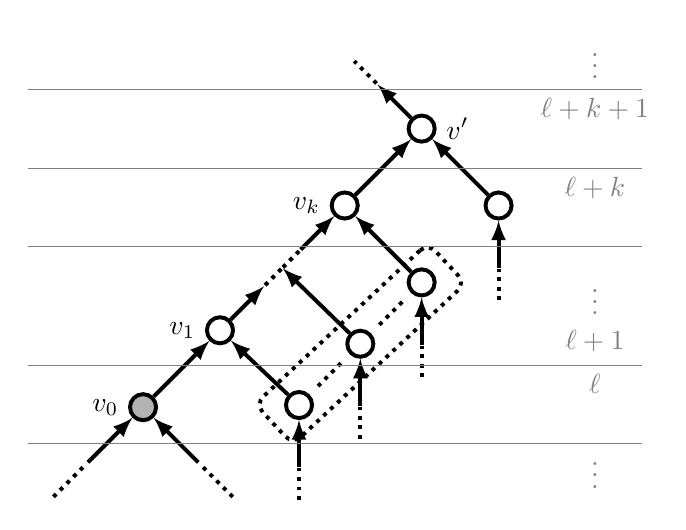
\begin{tikzpicture}
 \node[mynode,label=0:$v'$] (vp) {};
 \node[mynodee, above left=6mm of vp] (alvp) {};
 \node[mynodee, above left=4mm of alvp] (alalvp) {};
 \node[mynode, below left=10mm of vp, label=left:$v_k$] (vk) {};
 \node[mynodee, below left=6mm of vk] (vk-1) {};
 \node[mynodee, below left=3mm of vk-1] (vk-2) {};
 \node[mynodee, below left=3mm of vk-2] (vk-3) {};
 \node[mynode, below left=6mm of vk-3, label=left:$v_1$] (v1) {};
 \node[mynode, fill=black!30,below left=10mm of v1, label=left:$v_0$] (v0) {};
 \node[mynodee, below left=8mm of v0] (v00) {};
 \node[mynodee, below left=6mm of v00] (v000) {};
 \node[mynodee, below right=8mm of v0] (v01) {};
 \node[mynodee, below right=6mm of v01] (v011) {};
 \node[mynode, below right=10mm of vp] (rovp) {};
 \node[mynodee, below=6mm of rovp] (brovp) {};
 \node[mynodee, below=4mm of brovp] (bbrovp) {};
 \node[mynode, below right=10mm of vk] (rovk) {};
 \node[mynodee, below=6mm of rovk] (brovk) {};
 \node[mynodee, below=4mm of brovk] (bbrovk) {};
 \node[mynodee, below left=5mm of rovk] (rovk-1) {};
 \node[mynode, below left=2mm of rovk-1] (rovk-2) {};
 \node[mynodee, below=6mm of rovk-2] (brovk-2) {};
 \node[mynodee, below=4mm of brovk-2] (bbrovk-2) {};
 \node[mynodee, below left=2mm of rovk-2] (rovk-3) {};
 \node[mynode, below left=5mm of rovk-3] (rov1) {};
 \node[mynodee, below=6mm of rov1] (brov1) {};
 \node[mynodee, below=4mm of brov1] (bbrov1) {};
 \node[rect,rotate=43] at (rovk-2) (rect) {};

 \draw[dotted,line width=0.5mm] (v000) -- (v00);
 \draw[-latex,line width=0.5mm] (v00) -- (v0);
 \draw[-latex,line width=0.5mm] (v0) -- (v1);
 \draw[-latex,line width=0.5mm] (v1) -- (vk-3);
 \draw[dotted,line width=0.5mm] (vk-3) -- (vk-2);
 \draw[dotted,line width=0.5mm] (vk-2) -- (vk-1);
 \draw[-latex,line width=0.5mm] (vk-1) -- (vk);
 \draw[-latex,line width=0.5mm] (vk) -- (vp);
 \draw[-latex,line width=0.5mm] (vp) -- (alvp);
 \draw[dotted,line width=0.5mm] (alvp) -- (alalvp);
 \draw[-latex,line width=0.5mm] (rovp) -- (vp);
 \draw[-latex,line width=0.5mm] (brovp) -- (rovp);
 \draw[dotted,line width=0.5mm] (bbrovp) -- (brovp);
 \draw[-latex,line width=0.5mm] (rovk) -- (vk);
 \draw[-latex,line width=0.5mm] (rovk-2) -- (vk-2);
 \draw[-latex,line width=0.5mm] (rov1) -- (v1);
 \draw[-latex,line width=0.5mm] (v01) -- (v0);
 \draw[dotted,line width=0.5mm] (v011) -- (v01);
 \draw[-latex,line width=0.5mm] (brovk) -- (rovk);
 \draw[dotted,line width=0.5mm] (bbrovk) -- (brovk);
 \draw[-latex,line width=0.5mm] (brovk-2) -- (rovk-2);
 \draw[dotted,line width=0.5mm] (bbrovk-2) -- (brovk-2);
 \draw[-latex,line width=0.5mm] (brov1) -- (rov1);
 \draw[dotted,line width=0.5mm] (bbrov1) -- (brov1);
 \draw[dotted,line width=0.5mm,shorten >=1.5mm,shorten <=1.5mm] (rov1) -- (rovk-2);
 \draw[dotted,line width=0.5mm,shorten >=1.5mm,shorten <=1.5mm] (rovk-2) -- (rovk);

 \foreach \i/\l in {{-4/}, {-3/\ell}, {-1.5/}, {-.5/\ell+k}, {.5/\ell+k+1}} {
   \draw[very thin,gray] (-5,\i) -- (2.8,\i) node [below] at (2.2,\i) {$\l$};
  }
  \node[gray] at (2.2,.9) {$\vdots$};
  \node[gray] at (2.2,-2.1) {$\vdots$};
  \node[gray] at (2.2,-2.7) {$\ell+1$};
  \node[gray] at (2.2,-4.3) {$\vdots$};
\end{tikzpicture}

\end{document}
